\subsection{Controlled experiments: what makes training work}\label{sec:pilots}

We first trained single modes in the tight-coupling era, comparing each variant with the reference solver integrating the identical equations. Errors are $\max_\tau|X_{\rm PINN}-X_{\rm ref}|/\max_\tau|X_{\rm ref}|$ for each variable $X$; this metric is well defined through zero crossings, unlike pointwise relative error.

\paragraph{Output scaling.} With fixed per-variable scales the initial loss was $3\times10^{11}$ and training made no progress. The $1/(k\tau)^2$ factor in Eq.~\eqref{eq:phidot} amplifies any error in $\theta$ outside the horizon. Scaling the outputs by their super-horizon growth reduced the initial loss to $\mathcal{O}(1)$.

\paragraph{The constraint term.} At $k=0.01$\,Mpc$^{-1}$, up to $\tau=200$\,Mpc, training on the evolution residuals alone reached a lower ODE loss ($3.8\times10^{-6}$) than training with the $00$ term, yet its errors were 30 times larger: $2.7\times10^{-2}$ on $\phi$ against $9.7\times10^{-4}$ (Fig.~\ref{fig:pilot1}). Its error grows steadily after $\tau\sim10$\,Mpc, the signature of the constraint-violating solution of Sec.~\ref{sec:ics}. With the constraint term and a longer L-BFGS polish (12k steps), every variable reached $\le6\times10^{-4}$ ($\phi$: $8.5\times10^{-5}$) in 9 CPU-minutes. Causal weighting~\cite{Wang2022causal} at $\epsilon=1$ had no effect: the weights stayed $\approx1$.

\begin{figure*}
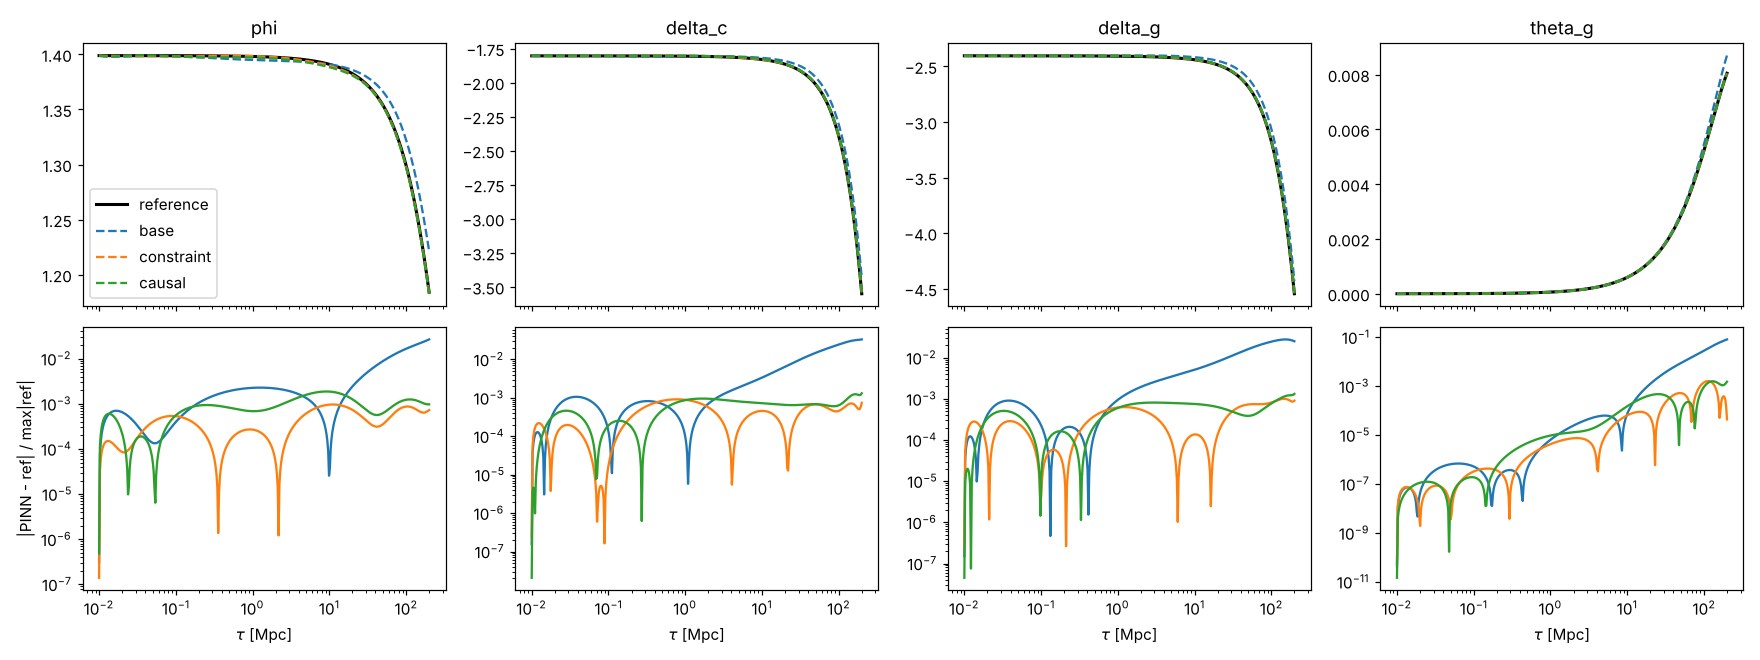
\includegraphics[width=\textwidth]{figures/pilot1.png}
\caption{Single mode $k=0.01$\,Mpc$^{-1}$, tight-coupling era. Top: PINN variants against the reference solver. Bottom: error normalised by $\max|X_{\rm ref}|$. Without the $00$ loss term (blue) the error grows steadily after $\tau\sim10$\,Mpc, despite a lower ODE residual.}
\label{fig:pilot1}
\end{figure*}

\paragraph{Oscillations and time-marching.} At $k=0.2$\,Mpc$^{-1}$, with the tight-coupling equations integrated to $\tau=200$\,Mpc (3.4 acoustic oscillations; a numerical stress test, since the TCA is not physically valid there), a single network failed with every error $\approx100\%$. It relaxed all variables towards zero from $\tau_i$ onwards (Fig.~\ref{fig:pilot2}, left), with or without the oscillation ansatz. Causal weighting at $\epsilon=10$ and $100$ did not help. This is not a problem of the equations or of capacity: the super-horizon segment alone ($\tau\le1$\,Mpc) trained to $\sim2\times10^{-3}$ at the same $k$. The single network gives up accuracy at early times to reduce the larger late-time oscillatory residual, a failure mode known for PINNs~\cite{Krishnapriyan2021}. Time-marching, with one window up to $k\tau=1$ and then one per acoustic period, chained by hard initial conditions~\cite{Wight2020,Krishnapriyan2021}, fixed it: every variable reached $\le1.0\times10^{-3}$, with no visible accumulation of error across the 8 windows (Fig.~\ref{fig:pilot2}, right). At $k=0.05$, where the TCA era holds half an oscillation, the oscillation ansatz improved a single network by $\approx2\times$.

\begin{figure*}
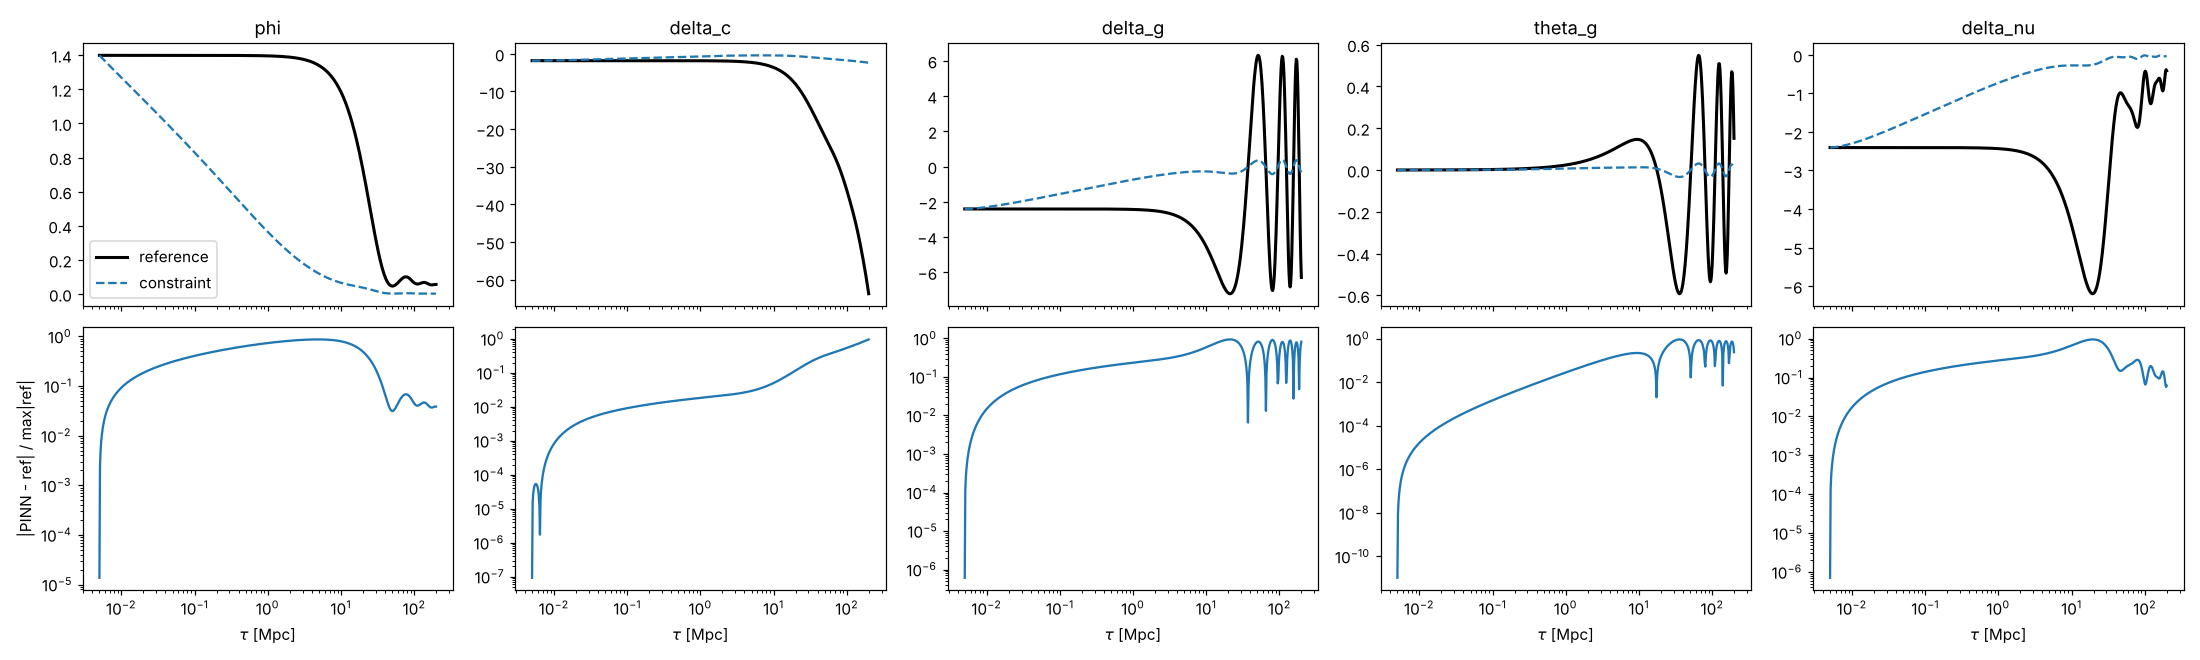
\includegraphics[width=0.49\textwidth]{figures/pilot2_single.png}\hfill
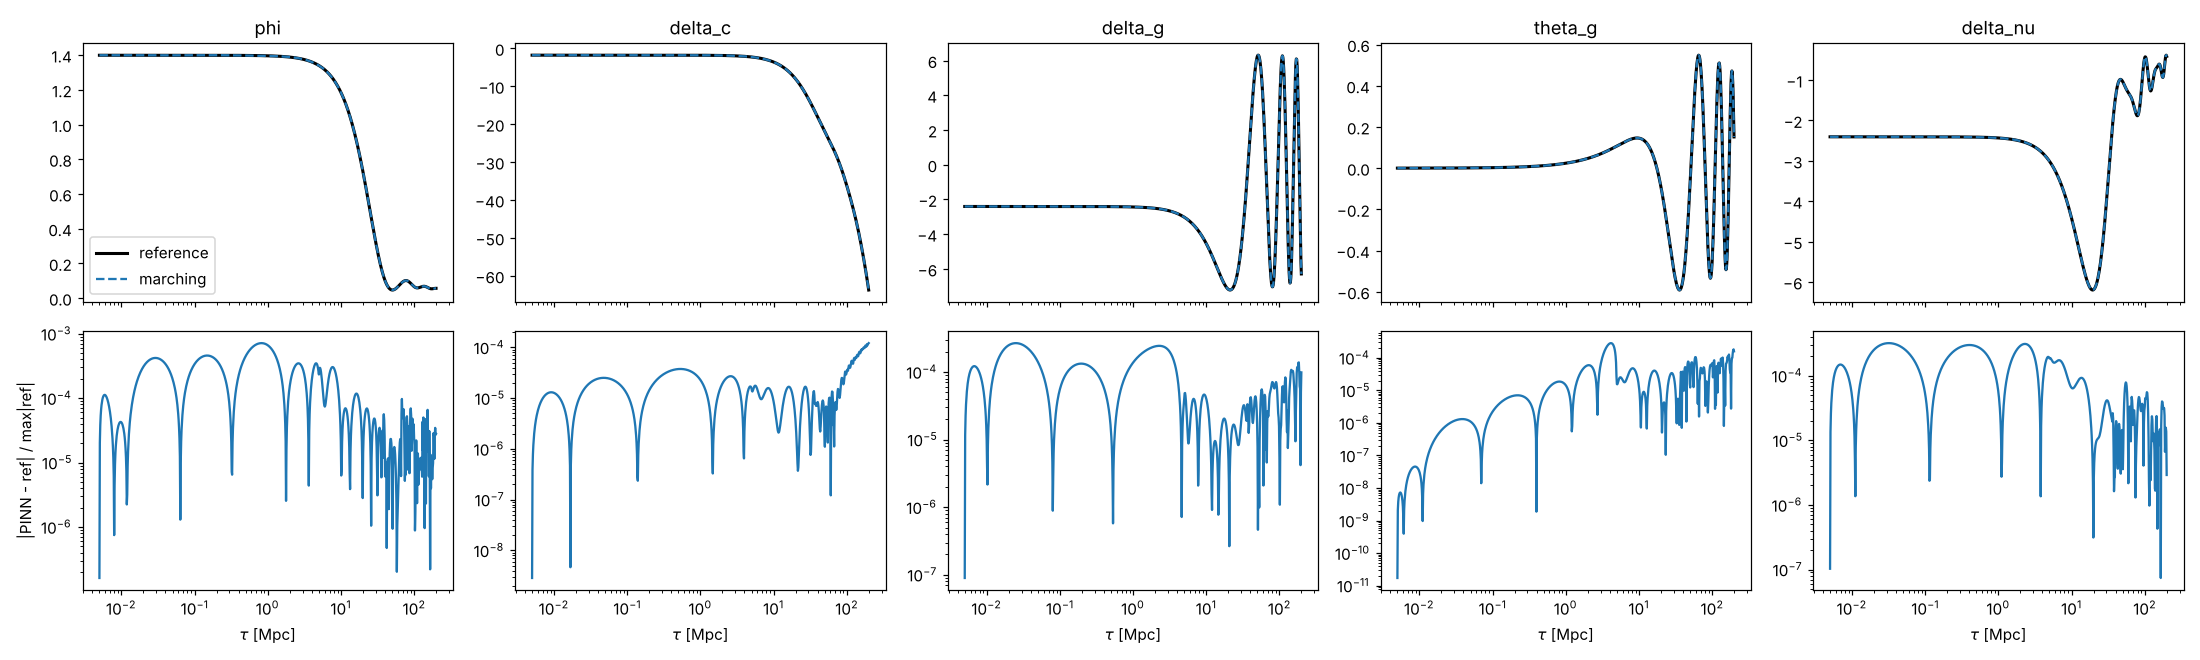
\includegraphics[width=0.49\textwidth]{figures/pilot2_marching.png}
\caption{$k=0.2$\,Mpc$^{-1}$ stress test through 3.4 acoustic oscillations. Left: a single network (with oscillation ansatz) collapses towards zero from the first time step. Right: time-marching over 8 windows; every variable is within $10^{-3}$ of the reference.}
\label{fig:pilot2}
\end{figure*}

\paragraph{The tight-coupling switch.} In a single-mode chain through recombination, the first full-hierarchy window trained to a loss of $6.7\times10^{-2}$, against $\sim5\times10^{-5}$ for every later window, when the state was handed over with zero baryon--photon slip. The full system relaxes to the quasi-static slip over $\delta\tau\sim1/\kd\approx0.01$\,Mpc, a boundary layer the network cannot represent. Handing over the first-order slip places the state on the slow manifold; the handed-over slip then matches the full system's to $10^{-4}$.

\subsection{Phase 1: wavenumber bundle in the tight-coupling era}\label{sec:phase1}

A three-window chain (edges $10^{-3}$, 1, 20, 200\,Mpc; 4$\times$64 networks with the oscillation ansatz; 20k Adam + 6k L-BFGS steps per window) was trained over $k\in[10^{-3},0.05]$\,Mpc$^{-1}$. It was evaluated on 20 held-out $k$, each up to its own TCA switch time. The RMS error over modes is $(0.9$--$2.2)\times10^{-3}$ across the variables, with maxima of $(1.7$--$5.1)\times10^{-3}$. The worst variable is the neutrino shear, and the worst mode is $k=0.033$. This misses the $10^{-3}$ target by a factor of 2--5. The error is already $\sim10^{-3}$ in the first, super-horizon window (Fig.~\ref{fig:phase1}), where the solution hardly depends on $k$. It therefore reflects accumulated residual error over a long window, not missing capacity for the $k$ dependence. Shorter windows, wider networks and second-order optimisers are the obvious remedies \pending{retrained Phase 1 chain}.

\begin{figure*}
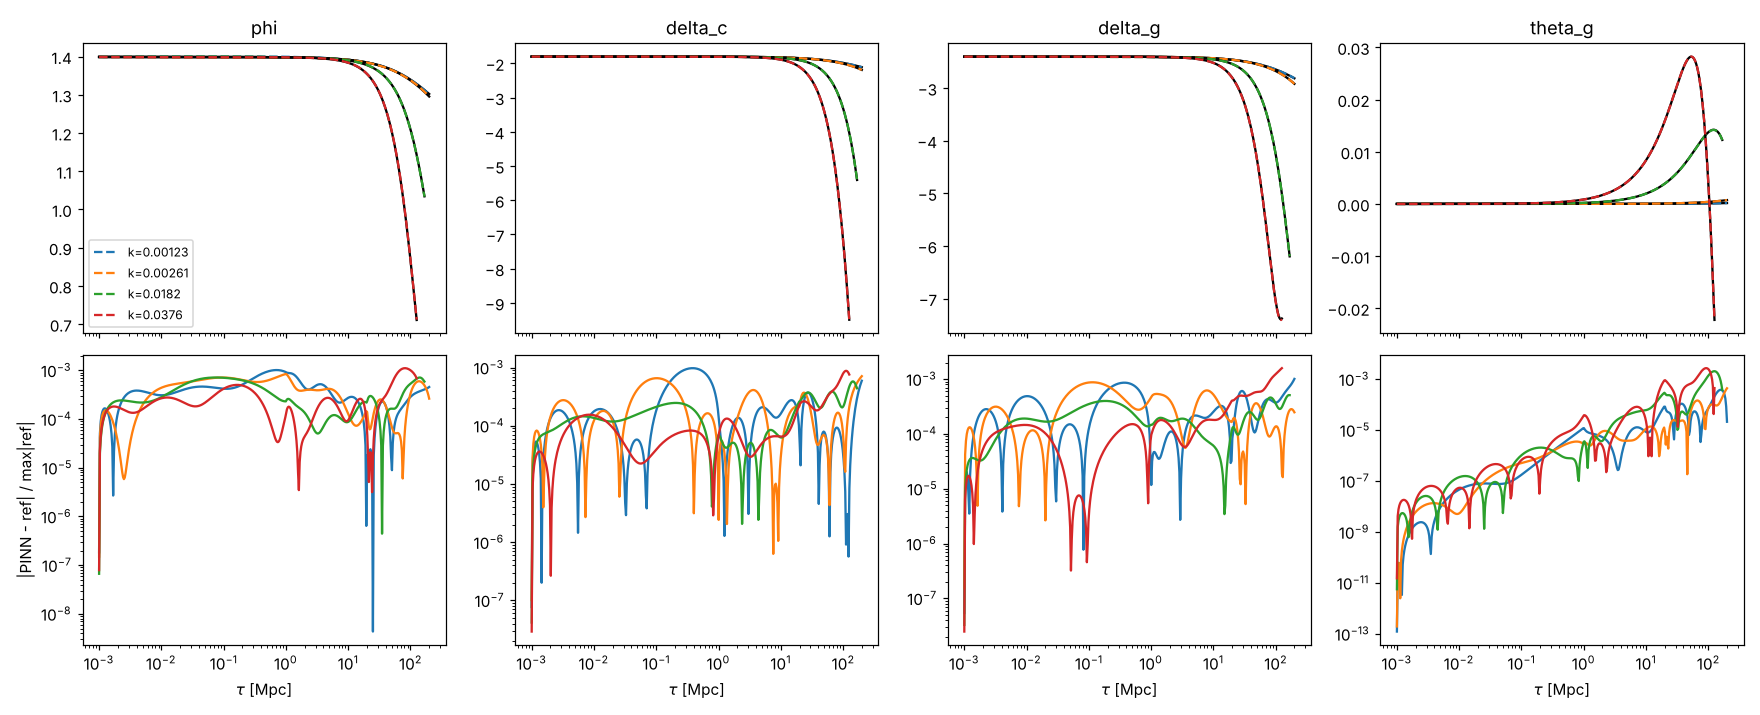
\includegraphics[width=\textwidth]{figures/phase1.png}
\caption{Phase 1 bundle over $k\in[10^{-3},0.05]$\,Mpc$^{-1}$: four of the 20 held-out modes. Bottom: error normalised by $\max|X_{\rm ref}|$.}
\label{fig:phase1}
\end{figure*}

\subsection{Phase 2: cosmological-parameter bundle}\label{sec:phase2}
\pending{bundle over $(k,\omega_b,\omega_c)\in[10^{-3},0.2]\times[0.020,0.024]\times[0.10,0.14]$ on the analytic background; held-out Latin hypercube of 30 points.}

\subsection{Phase 3: through recombination}\label{sec:phase3}
\pending{25-window chain (3 TCA, 19 full-hierarchy with $\ell_{\max}=12/10/17$, 3 per-mode RSA) over $k\in[5\times10^{-6},0.12]$\,Mpc$^{-1}$; errors against \textsc{class} up to $2\taurec$.}

\subsection{Phase 4: $C_\ell^{TT}$}\label{sec:phase4}
The approximation schedule matters before the network does. With reference-solver sources, the \textsc{class}-like schedule (TCA trigger; RSA per mode at $k\tau>45$) reproduces \textsc{class} $C_\ell^{TT}$ to $\le7.7\times10^{-3}$ for $\ell\le30$ and $\le2\times10^{-3}$ above. A $k$-independent RSA switch, which would let a bundle use fixed windows, fails at low $\ell$. Switching all modes at $\tau=850$\,Mpc gives $C_2$ wrong by a factor of 200, and at $\tau=1400$\,Mpc 13\% errors for $\ell\le5$; both are fine ($\le1\%$) above $\ell\sim30$. Low-$k$ modes never satisfy $k\tau>45$ and need the full hierarchy until today, which is why the PINN chain switches per mode. \pending{$C_\ell^{TT}$ from PINN source functions vs \textsc{class}, $\ell\le500$.}

\subsection{Phase 5: a late-time modification of gravity and an inverse problem}\label{sec:phase5}
We consider $\mu(a)=G_{\rm eff}/G=1+\mu_0\,\Omega_\Lambda(a)/\Omega_{\Lambda,0}$ multiplying $G$ in the perturbed Einstein equations, with an unchanged background. This phenomenological model is not available in standard \textsc{class}. Since $|\mu-1|<2\times10^{-5}|\mu_0|$ before $\tau=2400$\,Mpc, the Phase 3/4 chain is reused up to there, and only the later windows are retrained with $\mu_0\in[-0.5,0.5]$ as an extra input. In the reference solver, $\mu_0=0.3$ raises the comoving matter density today by $\approx1\%$ and the potential by $\approx10\%$, independently of scale. \pending{validation of the $\mu_0$ bundle; recovery of $\mu_0$ from mock $z=0$ matter and Weyl-potential spectra (1\% errors), PINN vs reference-solver likelihoods and their cost.}
